\documentclass[fontsize=10pt,paper=a4,bibliography=totoc]{scrartcl}

\usepackage[utf8]{inputenc}
\usepackage[ngerman]{babel}
\usepackage{amsmath}
\usepackage{graphicx}
\title{Gliederung für die Ausarbeitung}
\author{K. Franke, M. Dolgov, F. Achilles}
\begin{document}
\maketitle

\section{Stand der Technik}
Verfügbare Konzepte
Gesamtwirkungsgrad
Probleme

\section{Idee}
\subsection{Beschreibung}
\subsection{Erhoffte Vorteile}

\section{Beschreibung des Programms}
\subsection{Ablaufdiagramm (Top-Level)}
\subsection{Möglichkeiten und Grenzen}
 (versch. Breitengrade, über ein Jahr hinweg etc.)
\section{Gesamtaufbau}
\subsection{CAD-Modell mit allen Nebenaggregaten}
 (Antriebe: Sterling, Turbine)
\subsection{Verschiedene Generatorantriebe}
 (Stirling, Turbine)
\section{Kosten}
\section{Ergebnisse}


\section{Alles Mögliche}

\begin{align*}
	AirMass(\xi)=\frac{1}{\cos(\xi)}
\end{align*}

\begin{figure}
	\centering
	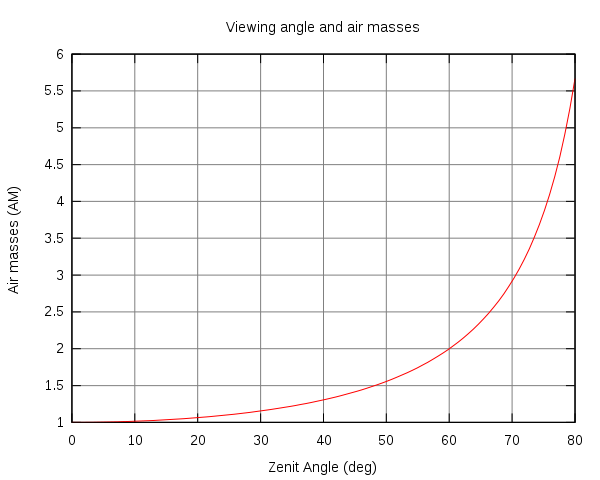
\includegraphics{images/Airmass.png}
	\caption{Luftmasse in Abhängigkeit vom Zenit-Winkel}
	\label{pic:AirMass}
\end{figure}

\begin{table}
\centering
	\caption{Werte für Strahlungsleistung. Wiki (engl) air mass solar energy. Stand 08.06.}
	\label{tab:airmass}
\begin{tabular}{|c|c|c|}
	\hline
	$\alpha$ & Air Mass & $\frac{W}{m^2}$\\
	\hline
	- & 0 & 1367\\
	\hline
	0 & 1 & 1040\\
	\hline
	23 & 1.09 & 1020\\
	\hline
	48.2 & 1.5 & 930\\
	\hline
	75 & 3.8 & 620\\
	\hline
	85 & 10 & 270\\
	\hline
\end{tabular}
\end{table}
Test
\begin{align*}
	I=1,1\cdot I_0 \cdot 0,7^{AM^{0,678}}
	\label{eqn:Intensity}
\end{align*}

\end{document}
